\begin{document}
Text
% Whole line comment

Text% Inline comment
\begin{comment}
This is an environment comment.
\end{comment}

This is a percent \%.
% Whole line comment without newline

\includegraphics{images/im1_included.png}
%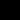
\includegraphics{images/im_not_included}

\includegraphics{images/include/images/im3_included.png}

\includegraphics{%
  images/im4_included.png%
  }
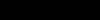
\includegraphics[width=.5\linewidth]{%
  images/im5_included.jpg}
%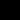
\includegraphics{%
%  images/im4_not_included.png
%  }
%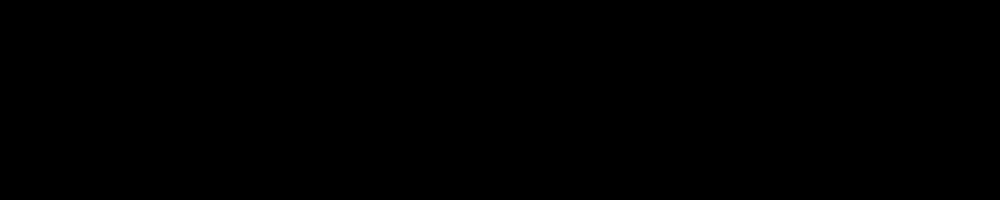
\includegraphics[width=.5\linewidth]{%
%  images/im5_not_included.jpg}

This line should\mytodo{Do this later} not be separated
\mytodo{This is a todo command with a nested \textit{command}.
Please remember that up to \texttt{2 levels} of \textit{nesting} are supported.}
from this one.

\newif\ifvar

\ifvar
\iffalse
\ifvar
Text
\fi
\fi
\fi

% content after this line should not be cleaned if \end{document} is in a comment

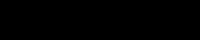
\includegraphics{images/im2_included.jpg}
\addplot{figures/data_included.txt}

% \addplot{figures/data_not_included.txt}
\input{figures/figure_not_included_2.tex}


% Test for tikzpicture feature
% should be replaced
\tikzsetnextfilename{test1}
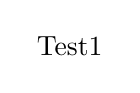
\begin{tikzpicture}
    \node (test) at (0,0) {Test1};
\end{tikzpicture}

% should be replaced in included file
\tikzsetnextfilename{test2}
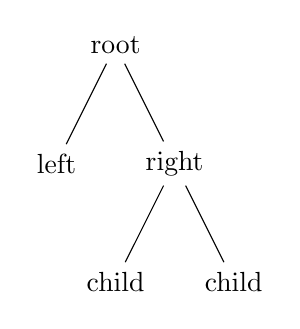
\begin{tikzpicture}
\node {root}
child {node {left}}
child {node {right}
child {node {child}}
child {node {child}}
};
\end{tikzpicture}

% should not be be replaced - no preceding tikzsetnextfilename command
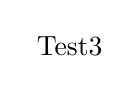
\begin{tikzpicture}
    \node (test) at (0,0) {Test3};
\end{tikzpicture}

\tikzsetnextfilename{test_no_match}
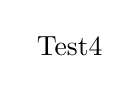
\begin{tikzpicture}
    \node (test) at (0,0) {Test4};
\end{tikzpicture}

\end{document}

This should be ignored.
